\documentclass{AsignaturaResumen}

\def\ISMAIN{1}
\SetTitulo{Fundamentos de bioprocesos}
\setabbreviationstyle[acronym]{long-short}
\makeglossaries

    % Glosario

\newglossaryentry{polimorfismo}{
    name={Polimorfismo},
    description={Existencia de dos o más variantes (alelos) de una secuencia de ADN en una población}
}
\newglossaryentry{locus}{
    name={Locus},description={Posición que ocupa un gen en el cromosoma}}
\newglossaryentry{amplicones}{
    name={Amplicones},
    description={Secuencias de ADN producidas por la amplificación de la hebra original en una \acrshort{pcr}. Se identifican como las bandas de una electroforesis en gel}
}
\newglossaryentry{sucesion microbiana}{
    name={Sucesión microbiana},
    description={Evento donde las especies de microorganismos presentes en una muestran son reemplazadas por otras}
}
\newglossaryentry{variante de secuencia}{
    name={Variante de Secuencia de Amplicón},
    description={Amplicón único de un conjunto de secuencias obtenidas en una secuenciación ya corregida}
}
\newglossaryentry{homopolimero}{
    name={Homopolímero},
    description={Secuencia repetitiva de nucleótidos (AGTGCGAT\emph{AAAA}TGCAGT, p.e.)}
}

    % Acrónimos

\newacronym{si}{SI}{Sistema Internacional}
\newacronym{iubmb}{IUBMB}{Unión Internacional de Bioquímica y Biología Molecular}

\newacronym{ros}{ROS}{especies reactivas de oxígeno}

\newacronym{pb}{pb}{pares de bases}
\newacronym{kb}{kb}{kilobases}

\newacronym{adn}{ADN}{Ácido desoxirribonucléico}
\newacronym{adnc}{ADNc}{ADN complementario}
\newacronym{dntps}{dNTPs}{desoxirribonucleótidos trifosfato}
\newacronym{ddntps}{ddNTPs}{didesoxinucleótidos}

\newacronym{adnpol}{ADNpol}{ADN polimerasa}

\newacronym{pcr}{PCR}{Reacción en Cadena de la Polimerasa}
\newacronym{rapd}{RAPD}{ADN Polimórfico Amplificado al Azar}
\newacronym{rflp}{RFLP}{Fragmentos de Restricción de Longitud Polimórfica}
\newacronym{dpcr}{dPCR}{PCR digital}
\newacronym{ngs}{NGS}{Secuenciación de Nueva Generación}
\newacronym{smrt}{SMRT}{Secuenciación en Tiempo Real de Molécula Única}

\newacronym{ccs}{CCS}{Lecturas de Consenso Circular}
\newacronym{asv}{ASV}{Variante de Secuencia de Amplicón}

\newacronym{iqi}{IQI}{Índice de Calidad Infaunal}

\newacronym{sds}{SDS}{dodecilsulfato sódico}
\newacronym{dms}{DMS}{dimetilsulfato}
\newacronym{ctab}{CTAB}{bromuro de cetiltrimetilamonio}

\begin{document}

    \frontmatter

\Portada
\Indices

    \mainmatter


\part{Introducción al desarrollo de bioprocesos}

    \chapter{Etapas del bioproceso e identificación de metabolitos} 


\section{Tipos de metabolitos}

\begin{itemize}
    \item Primarios
    \item Secundarios
\end{itemize}

\begin{itemize}
    \item Intracelulares
    \item Extracelulares
\end{itemize}

\section{Tipos de bioprocesos}

Podemos distinguir entre 2 tipos de bioprocesos: reactivos y extractivos.

\subsection{Bioprocesos reactivos}

En el caso de los bioprocesos reactivos, estos constan del uso de agentes biológicos (bacterias, hongos) para generar reacciones bioquímicas de interés.

Estos bioprocesos cuentan con 3 etapas:

\begin{enumerate}
    \item Upstream: Consta en la preparación de lo involucrado en la reacción, desde el microorganismo usado como del sutrato de este.
    \item Midstream o biorreacción: Es la reacción planeada, y es aquí donde se produce el producto de interés
    \item Downstream: Consiste en la separación del producto de interés del resto de sustancias no deseadas (microorganismos restantes, subproductos no deseados, etc.).
\end{enumerate}

\subsection{Bioprocesos extractivos}

Por otro lado, los procesos extractivos consisten en la extracción de productos ya existentes en el agente biológico de interés. Estos productos son lo que se conoce como metabolito.

Este tipo de bioprocesos, a diferencia de los reactivos, constan de solo 2 etapas:

\begin{enumerate}
    \item Upstream: Aquí se prepara la materia orgánica utilizada
    \item Downstream: En esta, después de la extracción, se busca purificar el metabolito de interés.
\end{enumerate}

Como se observar entonces al comparar los dos tipos de bioprocesos, la diferencia radica en la ausencia de una biorreacción en los procesos extractivos, y esto es por la naturaleza misma de tal tipo de bioproceso: solo consta de la obtención de compuestos que ya se encuentran presentes en el organismo.
    \chapter{Técnicas básicas de recuperación de productos} % ============================================================
% Capítulo 02: Técnicas básicas de recuperación de productos
% ============================================================

% Azúcares (totales y reductores) y producto

% Consejo: Este capítulo se enfoca en el Downstream. Explica cómo separar y purificar el producto de interés.

\section{Etapas del Downstream}

El \textbf{Downstream} o etapa de recuperación de productos es la fase final de un bioproceso y tiene como objetivo aislar, concentrar y purificar el producto de interés (metabolito) a partir del caldo de cultivo.

\begin{enumerate}
    \item \textbf{Separación mecánica de células:} Se eliminan las células y otros sólidos del líquido. Técnicas comunes incluyen:
        \begin{itemize}
            \item \textbf{Filtración:} Separación por tamaño usando membranas o filtros.
            \item \textbf{Centrifugación:} Separación por densidad usando fuerza centrífuga.
        \end{itemize}
    \item \textbf{Lisis celular:} Si el producto es intracelular, es necesario romper la pared y membrana celular para liberarlo. Técnicas:
        \begin{itemize}
            \item \textbf{Mecánicas:} Homogeneización a alta presión, molienda con perlas.
            \item \textbf{Químicas:} Uso de detergentes o solventes.
            \item \textbf{Enzimáticas:} Uso de enzimas como lisozima.
            \item \textbf{Físicas:} Choque osmótico, congelación-descongelación, ultrasonido.
        \end{itemize}
    \item \textbf{Concentración del producto:} Se reduce el volumen de la solución que contiene el producto. Técnicas:
        \begin{itemize}
            \item \textbf{Ultrafiltración:} Filtración con membranas de tamaño de poro específico para retener el producto y dejar pasar solvente.
            \item \textbf{Evaporación:} Eliminación del solvente por calor.
            \item \textbf{Extracción líquido-líquido:} Transferencia del producto a un solvente inmiscible.
        \end{itemize}
    \item \textbf{Purificación del producto:} Se busca obtener el producto con el mayor grado de pureza posible. Técnicas:
        \begin{itemize}
            \item \textbf{Cromatografía:} Separación basada en diferencias de afinidad, tamaño, carga o hidrofobicidad.
            \item \textbf{Precipitación:} Separación del producto de la solución añadiendo sales, solventes o cambiando el pH.
            \item \textbf{Cristalización:} Formación de cristales puros del producto.
        \end{itemize}
    \item \textbf{Acondicionamiento del producto:} Etapa final para darle la forma de presentación deseada (polvo, líquido, etc.).
\end{enumerate}

% Consejo: La estrategia de recuperación depende del tipo de metabolito (primario/secundario) y de su localización (intracelular/extracelular).

\section{Recuperación según el tipo de metabolito}

\begin{itemize}
    \item \textbf{Metabolitos extracelulares:} Son secretados al medio de cultivo. La recuperación es más sencilla, ya que no se requiere la lisis celular. Las etapas principales son la separación de células (filtración/centrifugación) y la purificación del producto desde el medio líquido.
    \item \textbf{Metabolitos intracelulares:} Permanecen dentro de la célula. Requieren una etapa de lisis celular para liberarlos, seguida de las etapas de concentración y purificación. Esto hace el proceso más complejo y costoso.
\end{itemize}

% Consejo: Para bioprocesos con células vegetales o animales, la lisis celular puede ser más delicada.

\subsection{Bioprocesos con células vegetales, animales y enzimas}

\begin{itemize}
    \item \textbf{Células vegetales y animales:} Son más frágiles que las bacterianas. La lisis celular se puede lograr con métodos suaves como la homogenización.
    \item \textbf{Enzimas:} Al ser proteínas, son sensibles a condiciones extremas de temperatura y pH. Se purifican típicamente por cromatografía de afinidad.
\end{itemize}
    \chapter{Técnicas básicas de cuantificación de biomasa} % ============================================================
% Capítulo 03: Técnicas básicas de cuantificación de biomasa
% ============================================================

%\section{Técnicas de cuantificación de biomasa}
%cuenta en placa
%cuenta en cámara
%nefelometría
%gravimetría

% Consejo: Este capítulo cubre cómo medir la cantidad de microorganismos en un cultivo.

\section{Técnicas de cuantificación de biomasa}

La cuantificación de biomasa es esencial para monitorear el crecimiento microbiano y el progreso del bioproceso.

\subsection{Cuenta en placa}
Es una técnica de cuantificación de células viables (vivas).
\begin{enumerate}
    \item Se realiza una serie de diluciones del cultivo.
    \item Se siembra una alícuota de cada dilución en una placa con medio de cultivo sólido.
    \item Se incuba y se cuentan las colonias que crecen.
    \item El número de colonias se multiplica por el factor de dilución para obtener el número de unidades formadoras de colonias (UFC/mL).
\end{enumerate}
% Consejo: Es muy precisa para células viables, pero es lenta y solo cuenta células que pueden crecer en el medio.

\subsection{Cuenta en cámara}
Es una técnica de cuantificación de células totales (vivas y muertas).
\begin{enumerate}
    \item Se coloca una muestra del cultivo en una cámara de conteo (hemocitómetro o cámara de Petroff-Hausser) que tiene una cuadrícula de volumen conocido.
    \item Se observa al microscopio y se cuentan las células en varios cuadros.
    \item Se calcula el número de células/mL usando un factor de conversión.
\end{enumerate}
% Consejo: Es rápida y sencilla, pero no distingue entre células vivas y muertas y puede ser imprecisa.

\subsection{Nefelometría (Turbidimetría)}
Es una técnica de cuantificación de células totales basada en la dispersión de la luz.
\begin{enumerate}
    \item Se mide la turbidez o absorbancia del cultivo en un espectrofotómetro a una longitud de onda específica (generalmente 600 nm).
    \item La absorbancia es proporcional a la concentración de biomasa.
    \item Se requiere una curva de calibración (absorbancia vs. peso seco) para obtener valores de concentración (g/L).
\end{enumerate}
% Consejo: Es una técnica rápida, sencilla y no destructiva, pero la absorbancia puede verse afectada por otros componentes del medio.

\subsection{Gravimetría}
Es una técnica de cuantificación de células totales basada en el peso seco.
\begin{enumerate}
    \item Se toma un volumen conocido del cultivo y se centrifuga para obtener un pellet celular.
    \item Se lava el pellet para eliminar residuos del medio.
    \item Se seca el pellet en una estufa hasta peso constante.
    \item Se pesa el pellet y se calcula la concentración de biomasa (g/L de peso seco).
\end{enumerate}
% Consejo: Es directa y precisa, pero es destructiva, consume tiempo y no es adecuada para muestras con baja concentración de biomasa.

\part{Estequiometría del crecimiento microbiano}

    \chapter{Estequiometría del crecimiento y balance elemental} 
Del griego \textit{stoikheion}, que significa ``elemento'', y \textit{métrón}, que significa ``medida'', la estequiometría consiste en el cálculo de las relaciones entre las cantidades de reactivos de una reacción química.

\section{Composición elemental de los microorganismos}

Los microorganismos cuentan con una composición elemental similar entre sí, por lo que esta puede ser promediada y utilizada para la estequiometría de reacciones microbianas.
Aunque la composición de macromoléculas de un organismo puede variar, la de los elementos apenas varía.


    \marginpar{\begin{minipage}{\marginparwidth}
        \begin{table}[H]\centering
    \caption{Composición elemental estándar de un microorganismo}
    \label{tab:composición_estándar_de_microorganismos}
    {\tabstyle
    \begin{tabular}{cc}\hline
        \theader{Elemento} & \theader{Porcentaje} \\ \hline
        
        C     & 46.5\%       \\
        H     & 6.49\%       \\
        O     & 31\%         \\
        N     & 10.85\%      \\
        Sales & $\approx$5\% \\    
    \hline\end{tabular}}
\end{table}
    \end{minipage}}


\section{Ejercicio 1 de balanceo de ecuaciones}

Podemos intentar balancear la siguiente ecuación, la cual representa la producción de ácido acético a partir de glucosa:

\begin{gather*}
    C_{6}H_{12}O_{6} + O_{2} + NH_{3} 
    \\
    \downarrow
    \\
    C_{0.039}H_{0.072}O_{0.021}N_{0.069} + C_{6}H_{8}O_{7} + CO_{2} + H_{2}O
\end{gather*}

Se puede notar rápidamente que intentar resolver este ejercicio ``al tanteo'' es complicado, si no imposible, por lo que es mejor recurrir al método algebráico, cuyo proceso se realiza de la siguiente manera:

\begin{enumerate}
    
    \item Definimos los coeficientes de cada compuesto en base a las letras del abecedario.\footnote{Se abrevia como Biomasa para ahorro de espacio.}
        \begin{equation*}
            \text{A}(C_{6}H_{12}O_{6}) + \text{B}(O_{2}) + \text{C}(NH_{3}) \Longrightarrow \text{D}(\text{Biomasa}) + \text{E}(C_{6}H_{8}O_{7}) + \text{F}(CO_{2}) + \text{G}(H_{2}O)
        \end{equation*}

    \item Luego, revisamos cuantas veces aparece cada elemento en cada compuesto de la ecuación química, y ordenamos como si fuera una ecuación matemática.
        \begin{enumerate}
	        \item Por ejemplo, iniciando con el carbono (C), tomamos que en el primer compuesto, la glucosa ($C_{6}H_{12}O_{6}$), hay 6 carbonos, y su coeficiente es A, por lo que tenemos que el primer término de la ecuación es $6A$. Esto lo repetimos con todos los compuestos de la ecuación que contengan carbono, y así obtendríamos la primera ecuación.
	        \item Este proceso lo repetimos con el resto de elementos ($H$, $O$ y $N$).
	        \item Un detalle a agregar es que cuando se está armando la ecuación se cambia la flecha de la ecuación química ($\Longrightarrow$) por un signo de igual ($=$).
        \end{enumerate}

    \item Terminaríamos con las siguientes ecuaciones:
        \begin{align*}
            C \quad &\longrightarrow \quad 6A = 0.39D + 6E + F
            \\
            H \quad &\longrightarrow \quad 12A + 3C = 0.72D + 8E + 2G
            \\
            O \quad &\longrightarrow \quad 6A + 2B = 0.021D + 7E + 2F + G
            \\
            N \quad &\longrightarrow \quad C = 0.0069D
        \end{align*}
\end{enumerate}

Esta nueva forma de ordenar los elementos nos permite despejar los distintos coeficientes de la ecuación química como si fuera cualquier otra ecuación matemática. Cada elemento representaría una ecuación y cada coeficiente una incógnita.

Ahora, antes de intentar despejar alguna incógnita, debemos recordar que una serie de ecuaciones sea posible de resolver debemos de tener la misma cantidad de ecuaciones y de incógnitas.\footnote{Recordar los grados de libertad de la materia Balance de Materia y Energía} En este caso tenemos 4 ecuaciones (Una por cada elemento, C, H, O y N) y 7 incógnitas (Cada letra del abecedario asignada), por lo que no es posible de resolver tal como está.

Afortunadamente, existen valores que pueden ayudar a modificar la ecuación de forma que sea posible de resolver, y estos son los rendimientos.

Los rendimientos reflejan la cantidad obtenida de ``algo'' tras la inversión de otro ``algo''. En bioprocesos el elemento invertido es el sustrato ($s$), mientras que los elementos obtenidos son biomasa ($x$) y un producto dado ($p$), como lo  puede ser el etanol. Así pues, tenemos dos rendimientos, $Y_{xs}$ y $Y_{ps}$.

\begin{equation*}
    Y_{xs} = \frac{\text{g de biomasa}}{\text{g de sustrato}} \quad ; \quad Y_{ps} = \frac{\text{g de producto}}{\text{g de sustrato}}
\end{equation*}

Donde: 

\begin{equation*}
    x = \text{Biomasa} \quad ; \quad s = \text{Sustrato} \quad ; \quad p = \text{Producto}
\end{equation*}

Estos valores, obtenidos a través de pruebas de laboratorios, nos pueden ayudar a despejar los coeficientes del sustrato, la biomasa y del producto (Ácido acético, $C_{6}H_{8}O_{7}$), dejando el conjunto de ecuaciones con 4 ecuaciones y 4 incógnitas, o sea, posible de resolver.

Para ello unicamente tomamos los rendimientos. En este caso supondremos que:

\begin{equation*}
    Y_{xs} = 0.153 \quad ; \quad Y_{ps} = 0.85
\end{equation*}

También también se necesitarán los pesos molares del sustrato, de la biomasa y del producto.

\begin{align*}
    PM_{s} = \frac{180g}{mol} \quad ; \quad PM_{x} = \frac{96.5g}{mol} \quad ; \quad PM_{p} = \frac{192g}{mol}
\end{align*}

Con estos datos, primero se establecerá el coeficiente correspondiente al sustrato ($A$) como 1, esto porque queremos saber cuanta biomasa y cuanto producto se generan a partir de 1 mol de sustrato.

\begin{gather*}
    \frac{0.153g_{x}}{1g_{s}} \cdot \frac{1mol_{x}}{96g_{x}} \cdot \frac{180g_{s}}{1mol_{s}} \cdot = 0.287\frac{mol_{x}}{mol_{s}}
    \\
    \\
    \frac{0.85g_{p}}{1g_{s}} \cdot \frac{1mol_{p}}{192g_{p}} \cdot \frac{180g_{s}}{1mol_{s}} \cdot = 0.797\frac{mol_{p}}{mol_{s}}
\end{gather*}

Teniendo ahora los coeficientes del sustrato, la biomasa y del producto, podemos reemplazarlos en la ecuación química y volver a realizar el balance algebráico

\begin{align*}
    1(C_{6}H_{12}O_{6}) + B(O_{2}) + C(NH_{3}) &\Longrightarrow 0.287(\text{Biomasa}) + 0.797(C_{6}H_{8}O_{7}) + F(CO_{2}) + G(H_{2}O)
    \\
    \\
    C &\longrightarrow 6(1) = 0.39(0.287) + 6(0.797) + F
    \\
    H &\longrightarrow 12(1) + 3C = 0.72(0.287) + 8(0.797) + 2G
    \\
    O &\longrightarrow 6(1) + 2B = 0.021(0.287) + 7(0.797) + 2F + G
    \\
    N &\longrightarrow C = 0.0069(0.287)
\end{align*}

Despues de realizar los cálculos deberíamos de tener:

\begin{align*}
    A&=1     & B&=2.43  & C&=0.002
    \\
    D&=0.287 & E&=0.797 & F&=1.238
    \\
    G&=2.8
\end{align*}

Y ordenando en la ecuación original tendríamos:

\begin{gather*}
    C_{6}H_{12}O_{6} + 2.43(O_{2}) + 0.002(NH_{3})
    \\
    \downarrow
    \\
    0.287(\text{X}) + 0.797(C_{6}H_{8}O_{7}) + 1.238(CO_{2}) + 2.8(H_{2}O)
\end{gather*}
    \chapter{Balance de electrones y grado de reducción} 


\section{Grados de reducción}



\section{Cálculo de los grados de reducción}


    \chapter{Formulación de medios de cultivo y relación C/N} 
Mucho del trabajo en biotecnología consta de hacer crecer a un microorganismo dado, y aunque pueden existir varios motivos para llevarlo a cabo, nada sería posible si el microorganismo no crece en primer lugar. Para no dejar este proceso en manos del azar, el crecimiento de estos microorganismos se lleva a cabo en medios de cultivo que se diseñan de manera que suplan al microorganismo de todos los elementos que requiere, y que así este crezca de la manera deseada. Estos medios de cultivo son preparados realizando una mezcla precisa de compuestos que son los que aportan los elementos. Si bien a veces cada compuesto aporta un elemento dado, en otras ocasiones diferentes compuestos pueden aportar el mismo elemento, o también es común que un compuesto aporte varios elementos a la vez. A pesar de que estos casos puedan parecer complicar el proceso de formulación, realmente apenas y es así, y al final la mezcla de todos los compuestos aporta la totalidad requerida de elementos en la proporción adecuada. La formulación de medios de cultivo consta pues en obtener cuanto se necesita agregar de cada compuesto para suplir las necesidades del microorganismo dado.

El proceso de la formulación de medios consta principalmente de los siguientes pasos:

\begin{enumerate}
    \item Definir la cantidad necesitada de cada elemento.
    \item Identificar que compuesto te aporta cada elemento.
    \item En base a la cantidad requerida de un elemento dado, calcular su equivalente en masa del compuesto que lo aporta.
\end{enumerate}

Existen un par de consideraciones a establecer para la formulación de medios de cultivo:

\begin{enumerate}
    \item Los elementos hidrógeno y oxígeno no son contemplados en los cálculos, esto porque tales elementos son suministrados por el agua del medio.
    \item Tanto en los casos donde un compuesto aporte varios elementos como cuando varios compuestos aportan el mismo elemento, solo es necesario elegir la masa más alta, puesto que con tal cantidad ya se suple la masa del otro compuesto.    
\end{enumerate}

\section{Ejercicio introductorio a formulación de medios} \label{sec:formulación_de_medios_ejemplo1} 

Todo esto puede quedar más claro con el siguiente ejercicio:

\begin{itemize}
    \item Diseñar un medio de cultivo con sulfato de amonio ($(NH_{4})_{2}SO_{4}$), fosfato de potasio ($K_{3}PO_{4}$), sulfato de magnesio ($MgSO_{3}$) y cloruro de calcio ($CaCL_{2}$), esto para producir 8.5 g/L de \textit{Pseudomonas fluorescens} a un pH de entre 6.5 a 7.5 y a una temperatura de 30°C en 15 litros de medio de cultivo.
    \item Se utiliza sacarosa como fuente de carbono, el nitrógeno es el nutriente limitante y los demás nutrientes deben estar en un exceso de 25\%.
    \item La composición celular es: 49.5\% C, 8\% H, 20\% O, 14.5\% N, 2.7\% P, 1\% S, 1\% K, 0.5\% Mg, 0.3\% Ca
\end{itemize}


En primer lugar, debemos identificar cuánto es necesario aportar de cada elemento, y para esto necesitamos la composición celular del microorganismo, lo cual nos dice qué porcentaje de la masa del microorganismo representa cada elemento en su composición. Podemos tomar de ejemplo el carbono, donde el 49.5\% indica que por cada gramo de \textit{P. fluorescens}, 0.495g son de carbono.

Para obtener la cantidad de carbono necesaria para el medio total solo necesitamos saber cuantos gramos de \textit{P. fluorescens} se buscan obtener, para lo cual necesitamos los litros de medio que se buscan preparar y los gramos de \textit{P. fluorescens} que queremos en cada litro de ese medio.

Todo esto se puede ordenar en la siguiente operación, además del ejemplo del carbono:\footnote{Recordando que: $S$=Sustrato, $X$=Biomasa y $P$=Producto}\footnote{Definiendo: $\text{Elem}$=Elemento y $\text{Comp}$=Compuesto}

\begin{equation}\label{eq:g_elemento}
    \frac{\text{gElem}}{\text{gX}} \cdot \frac{\text{gX}}{\text{Lt}} \cdot \text{Lt} = \text{gElem requeridos} \quad ; \quad \frac{0.495\text{gC}}{1\text{gX}} \cdot \frac{8.5\text{gX}}{1\text{Lt}} \cdot 15\text{Lt} = 63.11\text{gC}
\end{equation}

Estos serán los gramos de carbono ($\text{C}$) que el organismo necesita que le suministremos, sin embargo, esto no lo hacemos de forma directa, sino mediante un compuesto que sirva de fuente de carbono, en este caso la sacarosa. Por ello, debemos de calcular cuántos gramos de sacarosa necesitamos para suplir los gramos de carbono requeridos.

Para esto, hacemos uso de los pesos molares tanto del compuesto que aporta el elemento, como de los átomos del elemento a aportar presentes en el compuesto.

Por ejemplo, volviendo a la sacarosa, buscamos en primer lugar el peso molar de la sacarosa (342.3g), y luego contamos cuántos carbonos existen en la sacarosa, puesto que es el elemento que queremos aportar. Tenemos pues que hay 12 carbonos en la sacarosa, para lo que solo nos faltaría multiplicar el peso molecular del carbono ($\approx$12) por esos 12 átomos de carbono, lo cual nos da como resultado 144. Esto lo que nos dice es que por cada 342.3g de sacarosa que agreguemos estaríamos aportando 144g de carbono. Los cálculos anteriores nos dicen que en nuestro ejemplo necesitamos solo 63.11g de carbono, y para esto solo necesitamos una multiplicación como la siguiente:  

\begin{equation}\label{eq:g_compuesto}
    \text{gElem} \cdot \frac{\text{gComp}}{\text{gElem en Comp}} = \text{gComp} \quad ; \quad 63.11\text{gC} \cdot \frac{342.3\text{gSac}}{144\text{gC}} = 150\text{gSac}
\end{equation}

Por último, en ocasiones se busca que algunos elementos estén en exceso para que el microorganismo no se encuentre en condiciones de estrés tan fácilmente. Para obtener la cantidad de compuesto que se necesita para cumplir el exceso requerido, unicamente se necesita multiplicar los gramos requeridos de compuesto por tal exceso. Por ejemplo, en este caso nos piden un exceso de 25\%, por lo que se realiza la siguiente multiplicación: 

\begin{equation}\label{eq:g_exceso}
    \text{gComp} \cdot \text{Exceso} = \text{gComp en exceso} \quad ; \quad 150\text{gSac} \cdot 1.25 = 187.5\text{gSac}
\end{equation}

Usualmente se pide que todos los elementos de un medio de cultivo estén en exceso, por lo que este proceso se repetiría con todos los compuestos. Esto sin embargo no es así para los elementos limitantes. Estos son elementos que se busca que permanezcan en la cantidad justa para que el microorganismo pueda crecer. Cuando se especifica que algún elemento será el ``limitante'' lo único que se realiza es no multiplicar los gramos de compuesto por el exceso, y en su lugar agregar los gramos justos para suplir el elemento, los cuales son los ya obtenidos en la \autoref{eq:g_compuesto}.

El cálculo del resto de elementos y compuestos se recopila en la \autoref{tab:resultados_formulación_de_medios_ejemplo1}, la cual es también un ejemplo de formato que puede ayudar a organizar mejor los datos que uno va recopilando durante el proceso de la formulación.

    \begin{table}[H]

\centering
\caption{Resultados para la \autoref{sec:formulación_de_medios_ejemplo1}}
\label{tab:resultados_formulación_de_medios_ejemplo1}

\begin{threeparttable}
{\small\setstretch{1.35}

\begin{tabular}{M{0.15\linewidth}M{0.15\linewidth}M{0.15\linewidth}M{0.15\linewidth}M{0.15\linewidth}}\hline

    \theader{Compuesto} & \theader{Peso molar} & \theader{g de elemento requeridos} & \theader{g de compuesto requeridos} & \theader{g de compuesto en exceso} \\ \hline
    
    C$_{12}$H$_{22}$O$_{11}$ &    342g/mol & 63.11gC  &            150g           &   187.5g  \\
    (NH$_{4}$)$_{2}$SO$_{4}$ & 132.14g/mol & 18.49gN  &           87.26g          & LIMITANTE\tnote{1} \\
    K$_{3}$PO$_{4}$          & 212.27g/mol &  3.44gP  &  \textbf{23.55g}\tnote{2} &  29.44g   \\
                             &             &  1.28gK  &            2.32g          &  -------- \\
    MgSO$_{3}$               & 104.37g/mol &  1.28gS  &   \textbf{4.17g}\tnote{2} &   5.21g   \\
                             &             &  0.64gMg &            2.78g          &  -------- \\
    CaCl$_{2}$               & 110.98g/mol &  0.38gCa &            1.05g          &   1.31g   \\
    
    \hline
\end{tabular}}

\begin{tablenotes}\tiny % ex: \tntote{1} ... \item[1]
    \item[1] No se calculó el exceso porque es el elemento limitante, y se busca que esté solo en la cantidad justa.; 
    \item[2] Se eligió el valor más alto, pues tal cantidad de compuesto suple ambos elementos.
\end{tablenotes}

\end{threeparttable}
\end{table}

Ahora, algo que se puede observar es que tanto el fosfato de potasio ($K_{3}PO_{4}$) como el sulfato de magnesio ($MgSO_{3}$) aportan 2 elementos al mismo tiempo. Cuando tenemos este tipo de compuestos realizamos el proceso de la \autoref{eq:g_elemento} y la \autoref{eq:g_compuesto} con cada elemento que aporte el compuesto.

Por ejemplo, en el caso del $K_{3}PO_{4}$ se realizan los cálculos tanto para el potasio ($K$) como para el fósforo ($P$). Una vez realizados, tendremos por un lado la cantidad necesaria de $K_{3}PO_{4}$ para suplir el ($K$), así como también la cantidad de $K_{3}PO_{4}$ necesaria para suplir el fósforo ($P$). De entre estas dos, se tomará en cuenta la mas alta, en este caso la del fósforo (23.55g). Esto es así porque al agregar los 23.55g necesarios para suplir el fósforo se está cumpliendo también la necesidad de potasio del microorganismo, de hecho, hay potasio en exceso, pero esto no influye en el crecimiento del microorganismo. Lo mismo sucede en el caso del sulfato de magnesio ($MgSO_{3}$).
    \chapter{Predicción de rendimientos y coeficientes de rendimiento} % ============================================================
% Capítulo 07: Predicción de rendimientos y coeficientes de rendimiento
% ============================================================

% Consejo: Este capítulo se enfoca en cómo usar la estequiometría para predecir cuánto producto o biomasa se obtendrá de un sustrato.

\section{Predicción de rendimientos}

Los rendimientos son relaciones que nos indican la eficiencia con la que un sustrato se convierte en biomasa o producto. Se pueden predecir a partir de la ecuación estequiométrica balanceada del crecimiento microbiano.

\subsection{Rendimiento de biomasa respecto a sustrato ($Y_{X/S}$)}
Es la cantidad de biomasa producida por gramo de sustrato consumido.

\begin{equation}
    Y_{X/S} = \frac{\text{Biomasa producida (g)}}{\text{Sustrato consumido (g)}} = \frac{\Delta X}{\Delta S}
\end{equation}

\subsection{Rendimiento de producto respecto a sustrato ($Y_{P/S}$)}
Es la cantidad de producto producido por gramo de sustrato consumido.

\begin{equation}
    Y_{P/S} = \frac{\text{Producto producido (g)}}{\text{Sustrato consumido (g)}} = \frac{\Delta P}{\Delta S}
\end{equation}

% Consejo: En la práctica, estos rendimientos se obtienen experimentalmente. Sin embargo, el balance estequiométrico permite calcular rendimientos teóricos máximos.

\section{Coeficientes de rendimiento máximo teórico}

El \textbf{rendimiento máximo teórico} se calcula a partir de la estequiometría de la reacción, asumiendo que no hay formación de subproductos y que el sustrato se convierte completamente en biomasa o producto.

\subsection*{Ejemplo: Cálculo de rendimiento teórico de etanol a partir de glucosa}

La ecuación de la fermentación alcohólica es:

\[
C_6H_{12}O_6 \rightarrow 2 C_2H_5OH + 2 CO_2
\]

*   Masa molar de glucosa = 180 g/mol.
*   Masa molar de etanol = 46 g/mol.

Por cada 1 mol de glucosa (180 g), se producen 2 moles de etanol (2 * 46 = 92 g).

El rendimiento máximo teórico de etanol respecto a glucosa es:

\[
Y_{P/S} = \frac{92 \text{ g etanol}}{180 \text{ g glucosa}} = 0.511 \text{ g etanol / g glucosa}
\]

\section{Coeficientes de rendimiento real}

El \textbf{rendimiento real} es el que se obtiene experimentalmente en un bioproceso real.

\[
Y_{P/S}^{\text{real}} = \frac{P_{\text{obtenido}}}{S_{\text{consumido}}}
\]

Siempre es menor que el rendimiento máximo teórico debido a:
\begin{itemize}
    \item El uso de parte del sustrato para el mantenimiento celular.
    \item La producción de subproductos no deseados.
    \item La ineficiencia de los procesos metabólicos.
\end{itemize}    

\part{Cinética del crecimiento microbiano}

    \chapter{Cinéticas de crecimiento y generación de producto} 
La cinética del crecimiento bacteriano se encarga de estudiar el ritmo al que un cultivo dado de células crece a lo largo del tiempo.

Este ritmo de crecimiento puede variar en base a varios factores. Algunos de ellos pueden ser:

\begin{itemize}
    \item El tipo de sustrato y su disponibilidad.
    \item Las condiciones fisicoquímicas del ambiente (temperatura y pH, principalmente.).
    \item El tamaño de la población en el medio.
    \item Presencia de sustancias que aceleren o ralentizen el crecimiento bacteriano.
\end{itemize} 

\section{Curvas de crecimiento bacteriano}

El crecimiento típico de un microorganismo se describe en la conocida curva de crecimiento bacteriano, cuya ejemplificación podemos observar en la \autoref{fig:curva_crecimiento_bacteriano}. Esta se compone de las siguientes fases:

\begin{enumerate}
    \item Fase de latencia o lag: Las velocidades de reproducción y de muerte son iguales. Consta de una adaptación al medio. Se activan principalmente mecanismos de mantenimiento celular.
    \item Fase logarítmica o log: La velocidad de reproducción es mayor a la de muerte, por ende, hay un crecimiento rápido. Predomina la producción de metabolitos primarios.
    \item Fase estacionaria: Las velocidades de reproducción y de muerte son de nuevo iguales. Predomina la producción de metabolitos secundarios.
    \item Fase de muerte: Aquí la velocidad de muerte es ahora mayor a la de reproducción.
\end{enumerate}

\begin{figure}\centering
    \resizebox{\linewidth}{!}{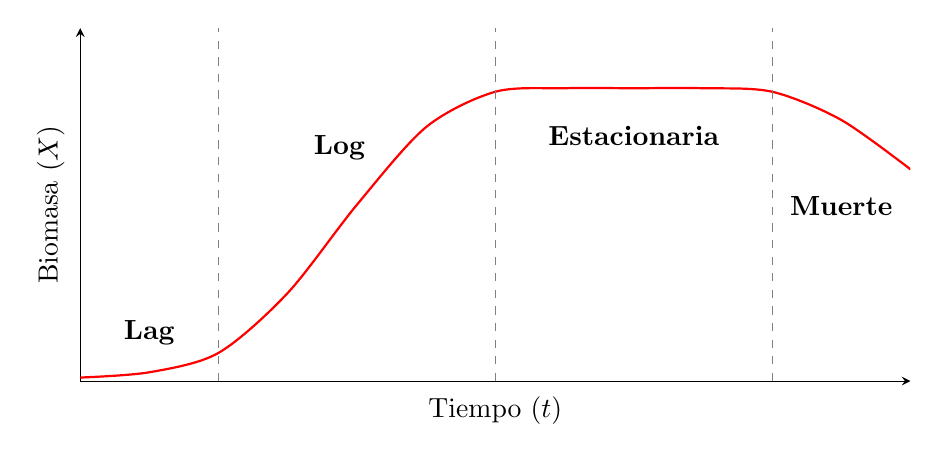
\begin{tikzpicture}
    \begin{axis}[
        width=\linewidth,
        height=0.5\linewidth,
        axis lines = left,
        xlabel = Tiempo ($t$),
        xmin=0, xmax=24,
        xtick=\empty,
        ylabel = Biomasa ($X$),
        ymin=0, ymax=10,
        ytick=\empty,
        grid=major,
        grid style={dashed, gray!20},
    ]
    \addplot[thick, red, smooth, tension=0.5] coordinates {
        (0, 0.1)      % Inoculación
        (2, 0.25)     % Fase lag
        (4, 0.8)
        (6, 2.5)
        (8, 5)      % Inicio fase log
        (10, 7.2)
        (12, 8.2)     % Mitad fase log
        (14, 8.3)
        (16, 8.3)     % Fin fase log
        (18, 8.3)     % Fase estacionaria
        (20, 8.2)
        (22, 7.4)     % Fase muerte
        (24, 6)
    };
    \draw[dashed, gray] (4,0) -- (4,10);
    \draw[dashed, gray] (12,0) -- (12,10);
    \draw[dashed, gray] (20,0) -- (20,10);
    \node[anchor=north] at (2,2) {\textbf{Lag}};
    \node[anchor=north] at (7.5,7.25) {\textbf{Log}};
    \node[anchor=north] at (16,7.5) {\textbf{Estacionaria}};
    \node[anchor=north] at (22,5.5) {\textbf{Muerte}};
    \end{axis}
\end{tikzpicture}}
    \rule{\linewidth}{0.5pt}
    \caption{Ejemplo de curva de crecimiento bacteriano}
    \label{fig:curva_crecimiento_bacteriano}
\end{figure}

En medios con múltiples sustratos, algunos microorganismos pueden mostrar múltiples fases logarítmicas, cada una con una fase estacionaria intermedia, en la cual el microorganismo realiza una serie de adaptaciones en su maquinaria enzimática para así poder degradar el nuevo sustrato. Un ejemplo de esto se muestra en la \autoref{fig:curva_diauxica}.
    
\begin{figure}\centering
    \resizebox{\linewidth}{!}{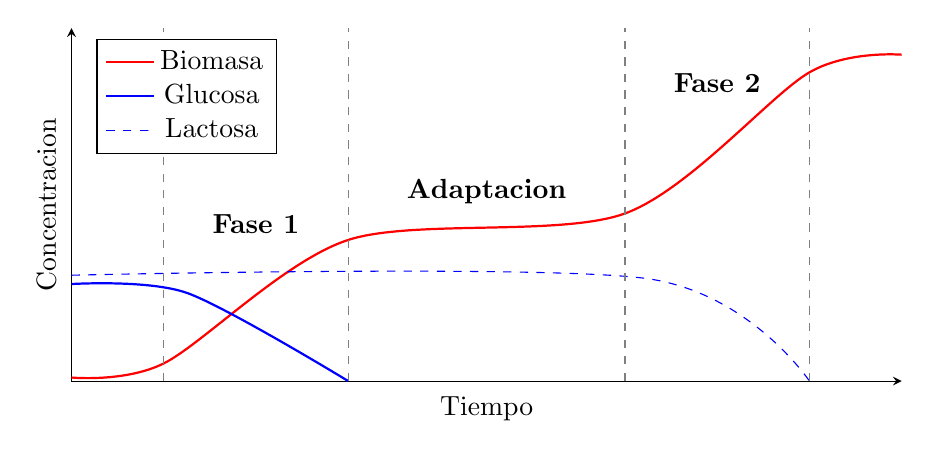
\begin{tikzpicture}
    \begin{axis}[
        width=\linewidth,
        height=0.5\linewidth,
        axis lines = left,
        xlabel = Tiempo,
        xmin=0, xmax=9,
        xtick=\empty,
        ylabel = Concentracion,
        ymin=0, ymax=10,
        ytick=\empty,
        grid=major,
        grid style={dashed, gray!20},
        legend pos=north west,
    ]
    \addplot[thick, red, smooth, tension=0.5] coordinates {
        (0, 0.1)
        (1, 0.5)
        (3, 4)
        (6, 4.75)
        (8, 8.75)
        (9, 9.25)
    };
    \addplot[thick, blue, smooth, tension=0.5] coordinates {
        (0, 2.75)
        (1.25, 2.5)
        (3, 0)
    };
    \addplot[dashed, blue, smooth, tension=0.5] coordinates {
        (0, 3)
        (6.25, 2.9)
        (8, 0)
    };
    \draw[dashed, gray] (1,0) -- (1,10);
    \draw[dashed, gray] (3,0) -- (3,10);
    \draw[dashed, gray] (6,0) -- (6,10);
    \draw[dashed, gray] (8,0) -- (8,10);
    \node[anchor=north] at (2,5) {\textbf{Fase 1}};
    \node[anchor=north] at (4.5,6) {\textbf{Adaptacion}};
    \node[anchor=north] at (7,9) {\textbf{Fase 2}};
    \addlegendentry{\textcolor{black}{Biomasa}}
    \addlegendentry{\textcolor{black}{Glucosa}}
    \addlegendentry{\textcolor{black}{Lactosa}}
    \end{axis}
\end{tikzpicture}}
    \rule{\linewidth}{0.5pt}
    \caption[Ejemplo de curva diáuxica]{Ejemplo de curva diáuxica. Se observa una correspondencia entre el consumo de glucosa y la primer fase log, así como del consumo de lactosa y la segunda fase log, así como una fase estacionaria intermedia, esto en el proceso para adaptar la maquinaria enzimática del microorganismo para poder degradar lactosa.}
    \label{fig:curva_diauxica}
\end{figure}


\section{Crecimiento exponencial de microorganismos}

Todas estas curvas son al final del día una representación gráfica del ritmo a la que los microorganismos se reproducen. Tal reproducción sigue un ritmo exponencial, esto porque los microorganismos al reproducirse parten de una célula para producir dos.\footnote{Así es para muchos microorganismos, más no para todos. Aún así, en bioprocesos se suele trabajar con microorganismos que siguen el típico crecimiento de fisión binaria.}. Vease por ejemplo la \autoref{fig:crecimiento_exponencial}.

Así pues, el crecimiento se puede representar con $2^{n}$, siendo $n$ el número de divisiones o generaciones que han transcurrido.

\begin{figure}\centering
    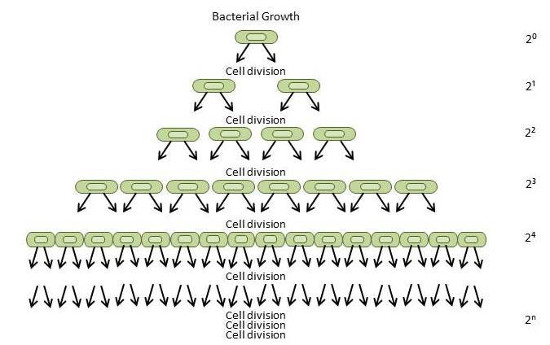
\includegraphics[width=\linewidth]{images/crecimiento_exponencial}
    \rule{\linewidth}{0.5pt}
    \caption[Representación gráfica del crecimiento exponencial bacteriano]{Representación gráfica del crecimiento exponencial bacteriano. Se puede apreciar el aumento del exponente de $2^{n}$ con cada división}
    \label{fig:crecimiento_exponencial}
\end{figure}

Tomando esto encuenta, podemos calcular la población en la que un cultivo de microorganismos se encuentra de la siguiente manera:

\begin{equation}\label{eq:nt}
    N_{t} = N_{0} \cdot 2^{n}
\end{equation}

Siendo $N_{0}$ la población con la que se inició, o población inicial, y $N_{t}$ la población actual del cultivo despues de pasadas las $n$ generaciones especificadas en $2^{n}$. 

Ahora, estos datos pueden graficarse de manera directa y se obtendría una linea exponencial sin embargo, puede resultar mejor aplicarles un logaritmo para obtener una linea recta, que puede ser estudiada con la respectiva ecuación de la recta ($y=mx+b$). Las diferencias entre ambas formas de graficar el crecimiento se muestran en la \autoref{fig:diferencias_grafica_directa_y_logaritmica}.


    \begin{figure}\centering
    \begin{subfigure}{0.45\linewidth}
        \begin{tikzpicture}
        \begin{axis}[
            width=\linewidth,
            height=\linewidth,
            axis lines = left,
            xlabel = {\tiny Generaciones ($n$)},
            xmin=0, xmax=10,
            xtick=\empty,
            ylabel = {\tiny No. de células ($N$)},
            ymin=0, ymax=1000,
            ytick=\empty,
        ]
        \addplot[thick, blue, domain=0:10, samples=40] {2^x};
        \end{axis}
        \end{tikzpicture}
        \rule{\linewidth}{0.5pt}
        \caption{Grafica directa}
        \label{fig:grafica_directa}
    \end{subfigure}
    \hspace{1em}
    \begin{subfigure}{0.45\linewidth}
        \begin{tikzpicture}
        \begin{axis}[
            width=\linewidth,
            height=\linewidth,
            axis lines = left,
            xlabel = {\tiny Generaciones ($n$)},
            xmin=0, xmax=10,
            xtick=\empty,
            ylabel = {\tiny No. de células ($log(N)$)},
            ymin=0, ymax=3,
            ytick=\empty,
        ]
        \addplot[thick, red, domain=0:10, samples=10] {log10(2^x)};
        \end{axis}
        \end{tikzpicture}
        \rule{\linewidth}{0.5pt}
        \caption{Grafica logaritmica}
        \label{fig:grafica_logaritmica}
    \end{subfigure}
    
    \vspace*{10pt}
    \rule{\linewidth}{0.5pt}
    \caption{Diferencia entre gráfica con número directo de bacterias y gráfica con escala logarítmica}
    \label{fig:diferencias_grafica_directa_y_logaritmica}
\end{figure}


\section{Tiempo de duplicación ($t_{d}$)}

Tal vez un elemento más importante en bioprocesos sea el tiempo de duplicación o generación, que se representa como $t_{d}$. Este representa el tiempo que un microorganismo necesita para duplicarse, y nos aporta información sobre qué tan rápido un cultivo crecerá. Se prefieren entonces tiempos de duplicación lo más bajos posibles cuando se trata de laproducción de biomasa o de la obtención de algún subproducto. Este valor se ve afectado por las condiciones del medio (sustrato, temperatura, pH, etcétera).

Para calcular el tiempo de duplicación de un microorganismo dado solo necesitamos el siguiente cálculo:

\begin{equation}
    t_{d} = \frac{t}{n}
\end{equation}

Siendo $t$ el tiempo que ha transcurrido y $n$ el número de generaciones que han transcurrido.

\section{Generaciones transcurridas ($n$)}

Ahora, en caso de no contar con el número de generaciones transcurridas podemos despejar la \autoref{eq:nt}:

\begin{align*}
    N_{t} = N_{0} \cdot 2^{n} \quad \longrightarrow \quad \log(N_{t}) = \log(N_{0}) - n \cdot \log(2) \quad \longrightarrow \quad \frac{\log(N_{t}) - \log(N_{0})}{\log(2)} = n
\end{align*}

Para obtener así:

\begin{equation}\label{eq:n}
    n = \frac{\log(N_{t}) - \log(N_{0})}{\log(2)}
\end{equation}

Es con esta ecuación que podemos obtener la generaciones que han pasado en un cultivo, unicamente haciendo uso de la población inicial y la población final.

\section{Cinética ($\mu$)}

Dado que la cinética estudia el cambio, a la cinética de crecimiento bacteriano le interesa saber el ritmo a la que un cultivo dado crece en distintos puntos del tiempo. El cambio en la cantidad de biomasa puede representarse con la siguiente ecuación:

\begin{equation*}
    r_{x} = \mu x
\end{equation*}

Esto también podemos expresarlo como una ecuación diferencial de la siguiente manera:

\begin{equation}\label{eq:ux}
    \frac{dx}{dt} = \mu x
\end{equation}

Esta nos dice cuanto cambia la cantidad de biomasa ($x$) respecto al tiempo ($t$). A su vez, $\mu$ es la velocidad específica a la que se da ese crecimiento bacteriano.

Para calcular $\mu$ solo necesitamos resolver la ecuación diferencial de la \autoref{eq:ux}, esto de la siguiente manera:

\begin{align*}
    \frac{dx}{dt} = \mu x & \longrightarrow \frac{1}{x} \ dx = \mu \ dt
    \\
    \\
    \int_{x_{0}}^{x}{\frac{1}{x}} \ dx = \int_{t_{0}}^{t_{d}}{\mu \ dt} &\longrightarrow \ln(x) - \ln(x_{0}) = \mu \cdot (t_{d} - 0)
\end{align*}

Despenjando tendríamos:

\begin{equation}
    \mu = \frac{\ln(x) - \ln(x_{0})}{t}
\end{equation}

Es con esta ecuación que podemos calcular $\mu$ unicamente haciendo uso de de las poblaciones de un cultivo dado ($x$ y $x_{0}$) y el tiempo transcurrido ($t$), y así saber a qué velocidad se está reproduciendo un microorganismo en un momento dado.
    \chapter{Modelado y cálculo de parámetros cinéticos} % ============================================================
% Capítulo 09: Modelado y cálculo de parámetros cinéticos
% ============================================================

% Consejo: Este capítulo se enfoca en los modelos matemáticos que predicen el comportamiento de los microorganismos en cultivo.

\section{Introducción al modelado cinético}

El modelado cinético permite predecir el comportamiento de un cultivo microbiano a lo largo del tiempo, incluyendo:
\begin{itemize}
    \item Crecimiento de biomasa ($X$)
    \item Consumo de sustrato ($S$)
    \item Formación de producto ($P$)
\end{itemize}

Existen diferentes enfoques para modelar estos procesos, que van desde los más simples hasta los más complejos y detallados.

\section{Modelos estructurados de predicción}

Los \textbf{modelos estructurados} consideran la composición intracelular de la biomasa. Dividen a la célula en diferentes componentes (ej. ADN, ARN, proteínas, lípidos, carbohidratos) y modelan la cinética de cada uno por separado.

\subsection{Características principales}
\begin{itemize}
    \item \textbf{Ventajas:}
        \begin{itemize}
            \item Son más precisos y realistas.
            \item Permiten predecir cómo cambia la composición celular en respuesta a cambios en el ambiente.
            \item Útiles para entender los mecanismos internos del metabolismo.
        \end{itemize}
    \item \textbf{Desventajas:}
        \begin{itemize}
            \item Son complejos matemáticamente.
            \item Requieren muchos parámetros que son difíciles de medir experimentalmente.
            \item Su implementación y calibración es costosa y demanda tiempo.
        \end{itemize}
\end{itemize}

\subsection{Ejemplo de modelo estructurado}

Un modelo estructurado simple podría dividir la biomasa en:

\begin{enumerate}
    \item Componente estructural (pared celular, membrana)
    \item Componente metabólico (enzimas, ARN)
    \item Componente de almacenamiento (glucógeno, lípidos)
\end{enumerate}

Cada componente tendría su propia ecuación de velocidad de formación/consumo.

% Consejo: En un curso de fundamentos, los modelos estructurados se introducen conceptualmente. Los modelos no estructurados son más prácticos para aplicaciones de ingeniería.

\section{Modelos no estructurados de predicción}

Los \textbf{modelos no estructurados} consideran a la biomasa como un "todo" uniforme y no distinguen sus componentes internos. Son los más utilizados en la práctica de la ingeniería de bioprocesos.

\subsection{Características principales}
\begin{itemize}
    \item \textbf{Ventajas:}
        \begin{itemize}
            \item Son simples y fáciles de usar.
            \item Requieren pocos parámetros.
            \item Son suficientes para describir el comportamiento global del cultivo.
        \end{itemize}
    \item \textbf{Desventajas:}
        \begin{itemize}
            \item No consideran cambios en la composición celular.
            \item Pueden no ser precisos en condiciones donde la fisiología celular cambia drásticamente.
        \end{itemize}
\end{itemize}

\subsection{Modelo de Monod}

Es el modelo no estructurado más común y relaciona la velocidad específica de crecimiento ($\mu$) con la concentración del sustrato limitante ($S$).

\begin{equation}
    \mu = \mu_{max} \frac{S}{K_S + S}
    \label{eq:monod}
\end{equation}

Donde:
\begin{itemize}
    \item $\mu$ es la velocidad específica de crecimiento (h$^{-1}$).
    \item $\mu_{max}$ es la velocidad específica de crecimiento máxima (h$^{-1}$).
    \item $S$ es la concentración del sustrato limitante (g/L).
    \item $K_S$ es la constante de saturación de Monod (g/L), que representa la concentración de sustrato a la que $\mu = \frac{1}{2} \mu_{max}$.
\end{itemize}

\subsection{Otros modelos no estructurados}

Existen variaciones del modelo de Monod para describir diferentes comportamientos:

\begin{itemize}
    \item \textbf{Inhibición por sustrato:} Cuando altas concentraciones de sustrato inhiben el crecimiento.
    \begin{equation}
        \mu = \mu_{max} \frac{S}{K_S + S + \frac{S^2}{K_I}}
    \end{equation}
    Donde $K_I$ es la constante de inhibición.
    
    \item \textbf{Inhibición por producto:} Cuando el producto acumulado inhibe el crecimiento.
    \begin{equation}
        \mu = \mu_{max} \frac{S}{K_S + S} \left(1 - \frac{P}{P_{max}}\right)
    \end{equation}
    Donde $P$ es la concentración de producto y $P_{max}$ es la concentración máxima tolerable.
    
    \item \textbf{Modelo de Tessier:} $\mu = \mu_{max}(1 - e^{-S/K_S})$
    \item \textbf{Modelo de Moser:} $\mu = \mu_{max} \frac{S^n}{K_S + S^n}$
\end{itemize}

% Consejo: El modelo de Monod es el más importante y el que se utiliza como base en la mayoría de los bioprocesos.

\section{Parámetros cinéticos en sistemas de producción}

Los sistemas de producción se clasifican según el modo de operación del biorreactor:

\subsection{Cultivo en lote (Batch)}
\begin{itemize}
    \item Todos los nutrientes se añaden al inicio.
    \item No hay entrada ni salida de material durante la operación.
    \item Las concentraciones de biomasa, sustrato y producto cambian con el tiempo.
    \item Parámetros a determinar: $\mu_{max}$, $K_S$, $Y_{X/S}$, $Y_{P/S}$, $q_S$, $q_P$.
\end{itemize}

\subsection{Cultivo en lote alimentado (Fed-batch)}
\begin{itemize}
    \item Se añade sustrato de forma continua o intermitente durante la operación.
    \item Permite mantener bajas concentraciones de sustrato para evitar inhibición.
    \item El volumen aumenta con el tiempo.
    \item Parámetros a determinar: $\mu_{max}$, $K_S$, $Y_{X/S}$, velocidad de alimentación.
\end{itemize}

\subsection{Cultivo continuo}
\begin{itemize}
    \item Hay entrada continua de medio fresco y salida continua de caldo de cultivo.
    \item Se alcanza un estado estacionario donde las concentraciones no cambian con el tiempo.
    \item Tipos: Quimiosato (control por dilución) y Turbidostato (control por biomasa).
    \item Parámetros a determinar: $\mu = D$ (velocidad de dilución), $Y_{X/S}$, productividad.
\end{itemize}

\section{Cálculo de parámetros cinéticos}

\subsection{Velocidad específica de crecimiento ($\mu$)}
Se calcula a partir de datos de biomasa en la fase exponencial:

\begin{equation}
    \mu = \frac{\ln(X) - \ln(X_0)}{t - t_0}
\end{equation}

\subsection{Rendimientos}
\begin{itemize}
    \item Rendimiento de biomasa: $Y_{X/S} = \frac{\Delta X}{\Delta S}$
    \item Rendimiento de producto: $Y_{P/S} = \frac{\Delta P}{\Delta S}$
    \item Rendimiento de producto respecto a biomasa: $Y_{P/X} = \frac{\Delta P}{\Delta X}$
\end{itemize}

\subsection{Velocidades específicas}
\begin{itemize}
    \item Velocidad específica de consumo de sustrato: $q_S = \frac{1}{X} \frac{dS}{dt}$
    \item Velocidad específica de formación de producto: $q_P = \frac{1}{X} \frac{dP}{dt}$
\end{itemize}

\subsection{Determinación de $K_S$ y $\mu_{max}$}
Se puede realizar mediante:
\begin{enumerate}
    \item Linealización de la ecuación de Monod (doble recíproca):
    \begin{equation}
        \frac{1}{\mu} = \frac{K_S}{\mu_{max}} \frac{1}{S} + \frac{1}{\mu_{max}}
    \end{equation}
    \item Ajuste no lineal de datos experimentales usando software especializado.
\end{enumerate}

\section{Estado estacionario y pseudoestacionario}

\subsection{Estado estacionario}
\begin{itemize}
    \item Ocurre en cultivos continuos (quimiosato).
    \item Las concentraciones de biomasa, sustrato y producto permanecen constantes en el tiempo.
    \item $\frac{dX}{dt} = \frac{dS}{dt} = \frac{dP}{dt} = 0$
    \item $\mu = D$ (velocidad de dilución)
\end{itemize}

\subsection{Estado pseudoestacionario}
\begin{itemize}
    \item Ocurre en cultivos en lote alimentado.
    \item La biomasa aumenta lentamente, pero la concentración de sustrato se mantiene constante.
    \item $\frac{dS}{dt} \approx 0$
    \item $\mu \approx \text{constante}$
\end{itemize}

% Consejo: Entender estos conceptos es fundamental para el diseño y operación de biorreactores a escala industrial.

\section{Ejercicio de aplicación}

\textbf{Problema:} Se tienen los siguientes datos de un cultivo en lote de \textit{E. coli} en medio con glucosa como sustrato limitante:

\begin{table}\centering
    \caption{Datos de cultivo en lote}
    \label{tab:datos_cultivo}
    \begin{tabular}{c|c|c|c}
        \textbf{Tiempo (h)} & \textbf{Biomasa (g/L)} & \textbf{Sustrato (g/L)} & \textbf{Producto (g/L)} \\
        \hline
        0 & 0.5 & 20.0 & 0.0 \\
        1 & 0.8 & 18.5 & 0.2 \\
        2 & 1.3 & 16.0 & 0.5 \\
        3 & 2.1 & 12.0 & 0.9 \\
        4 & 3.4 & 6.0 & 1.5 \\
        5 & 4.5 & 2.0 & 2.0 \\
        6 & 4.8 & 1.0 & 2.3 \\
        7 & 4.9 & 0.5 & 2.5 \\
        8 & 4.9 & 0.2 & 2.6 \\
    \end{tabular}
\end{table}

Calcular:

\begin{enumerate}
    \item La velocidad específica de crecimiento máxima ($\mu_{max}$) durante la fase exponencial.
    \item Los rendimientos $Y_{X/S}$ y $Y_{P/S}$.
    \item La velocidad específica de consumo de sustrato ($q_S$) al tiempo 4 h.
\end{enumerate}

\textbf{Solución:}

1. \textbf{Cálculo de $\mu_{max}$:} Usando los datos de la fase exponencial (tiempos 0-4 h):

\begin{align*}
    \mu &= \frac{\ln(X_2) - \ln(X_1)}{t_2 - t_1} \\
    \mu_{max} &= \frac{\ln(3.4) - \ln(0.5)}{4 - 0} = \frac{1.224 - (-0.693)}{4} = \frac{1.917}{4} = 0.479 \text{ h}^{-1}
\end{align*}

2. \textbf{Cálculo de rendimientos:}
\begin{align*}
    Y_{X/S} &= \frac{\Delta X}{\Delta S} = \frac{4.9 - 0.5}{20.0 - 0.2} = \frac{4.4}{19.8} = 0.222 \text{ g biomasa/g sustrato} \\
    Y_{P/S} &= \frac{\Delta P}{\Delta S} = \frac{2.6 - 0.0}{20.0 - 0.2} = \frac{2.6}{19.8} = 0.131 \text{ g producto/g sustrato}
\end{align*}

3. \textbf{Cálculo de $q_S$ al tiempo 4 h:}
\begin{align*}
    q_S &= -\frac{1}{X} \frac{dS}{dt} \approx -\frac{1}{3.4} \frac{(2.0 - 6.0)}{(5 - 3)} = -\frac{1}{3.4} \frac{(-4.0)}{2} = \frac{2.0}{3.4} = 0.588 \text{ g sustrato/(g biomasa·h)}
\end{align*}

\section{Simulación de bioprocesos}

La simulación computacional es una herramienta poderosa para:
\begin{itemize}
    \item Predecir el comportamiento del cultivo antes de realizar experimentos.
    \item Optimizar las condiciones de operación.
    \item Escalar el proceso de laboratorio a planta piloto o industrial.
    \item Evaluar diferentes estrategias de operación.
\end{itemize}

% Consejo: Existen software especializados como MATLAB, Aspen Plus, o simuladores específicos para bioprocesos. También hay recursos en línea como el "Virtual Labs project" mencionado en el manual.

\subsection{Elementos de una simulación}
\begin{enumerate}
    \item Modelo matemático (ej. ecuaciones de Monod, balances de masa).
    \item Parámetros cinéticos y estequiométricos.
    \item Condiciones iniciales.
    \item Condiciones de operación (temperatura, pH, agitación, etc.).
    \item Resolución numérica de las ecuaciones diferenciales.
\end{enumerate}


    \PlainGeom
    \appendix



    \backmatter

\Bibliografia
\Glosarios

\end{document}